\lecture{13}{11.04}
KNN算法的局限
\begin{itemize}
    \item 对参数选择很敏感
    \item 计算量大
\end{itemize}
当$K$ 值较小:易发生过拟合,受噪声影响较大

当$K$ 值太大:无法区分不同样本
\subsubsection{归一化}%
\label{subsub:归一化}
\begin{table}[htpb]
    \centering
    \caption{分类}
    \label{tab:分类}
    \begin{tabular}{|c|c|c|c|c|c|}
    \hline
    样本名 & $x_1$ & $x_2$ & $x_3$ & 类型 & $S_n$距离 \\
    \hline
    $S_1$ & 39 & 0 & 21 & $K_1$ & $\sqrt[3]{4133}\approx 16.05 $\\
    \hline
    $S_2$ & 3 & 5 & 65 & $K_2$ & $6\sqrt[3]{5^2} \sqrt[3]{19}\approx 46.81 $\\
    \hline
    $S_3$ & 21 & 17 & 5 & $K_1$ & $2\sqrt[3]{3^2} \sqrt[3]{14}\approx 10.03 $\\
    \hline
    \multicolumn{6}{|c|}{$\ldots $} \\
    \hline
    $S_n$ & 23 & 3 & 17 & ? & 0\\
    \hline
    \end{tabular}
\end{table}
特征值标准一致时无需归一化
\begin{notation}
    欧几里得距离:\[
        S=\sqrt{\sum_{i=1}^{n} \left( x_{i}^{(P)}-x_{i}^{(Q)} \right) ^2} 
    .\] 
    曼哈顿距离:\[
        S=\sum_{i=1}^{n} \left| x_{i}^{(P)}-x_{i}^{(Q)} \right| 
    .\] 
    切比雪夫距离:\[
        S=\underset{l}{\max}\left( \left| x_{i}^{(P)}-x_{i}^{(Q)} \right|  \right) 
    .\] 
\end{notation}
\subsubsection{决策树}%
\label{subsub:决策树}
\begin{defi}
    树形结构,由节点和边组成
\end{defi}
基本思想:一个if-then的规则集合

可以分为树形或细胞型
\begin{center}
    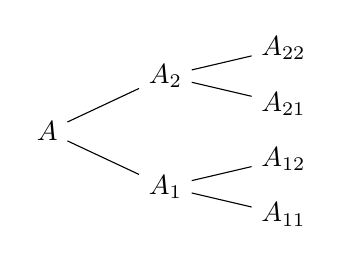
\begin{tikzpicture}[
        grow=right,
        level 1/.style={sibling distance=4em},
        level 2/.style={sibling distance=2em}
        ]
        \node [] (A) {$A$}
            child {node {$A_1$}
                child {node {$A_{11}$}}
                child {node {$A_{12}$}}
            }
            child {node {$A_2$}
                child {node {$A_{21}$}}
                child {node {$A_{22}$}}
            };
    \end{tikzpicture}
\end{center}
\begin{eg}
    ID3算法
\end{eg}
\subsection{无监督学习}%
\label{sub:无监督学习}
\begin{notation}
    区别:有监督学习中提供样本的标签,无监督学习中机器自行提取样本的相似性
\end{notation}
通过样本可以提取颜色、纹理、频率等特征

无监督函数通过定义相似度计算函数来提取特征的相似性,根据选择的相似度函数来分类
\begin{notation}
    K-均值聚类算法
\end{notation}
\section*{监督学习补充:线性回归\textit{Linear regression} }%
\label{sec:监督学习补充:线性回归}
\begin{defi}
    回归与分类:挖掘和学习输出变量和输入变量之间的潜在关系模型

    回归为连续、分类为离散
\end{defi}
\begin{eg}
    高尔顿提出衰退(regression, 回归)效应,指出:\[
        y=33.73+0.516 \frac{x_1+x_2}{2} 
    .\] 
    其中$x_1,x_2$ 为父母身高(单位:inch),$y$ 为经过回归后的下一代身高
\end{eg}
\begin{notation}
    最小二乘法:求出使残差平方和最小的$a,b$
\end{notation}




